\section{Experimental Dataset}

\subsection{Mobile Phone Data Source}
\label{subsec:mobiledatasource}

\subsubsection{Dataset Description}

The data used in this study consist of a multiset $P$ of composed of voice calls, and another multiset $S$ composed of text messages from a Mexican telecommunication company (\textit{telco}) for a 3 month period. These two sets are referred as the \emph{Call Detail Records}, or CDRs.

Every call $p \in P$ contains the phone numbers of the caller and callee $\left< p_o, p_d \right>$, which are anonymized using a cryptographic hash function for privacy reasons, the starting time $p_t$, and the call duration $p_s$. The same datum, except for the call duration, can be found for each element $s \in S$.

Additionally, the latitude and longitude of the antenna used for each call and SMS $\left< p_y, p_x \right>$  are given for certain users $V'$. Subsets $P' \subseteq P$ and $S' \subseteq S$ contain those calls.

Given that our collections $P$ and $S$ of CDRs are coming from one telephone company, we are able to reconstruct all communication links between clients of this company $N$, as well as communications between the clients and other users. However, we have no information on communications where neither users are clients of our telco company, and therefore users not in $N$ don't have complete call information.

The \emph{Communications Graph} $G = \left< V, E \right>$ is composed of he set of nodes $V = P_o \cup P_d \cup S_o \cup S_d$, and the set of directed edges $E$, where each element $e \in E$ is composed of an origin and destination $\left< e_o, e_d \right>$, the total amount of calls between these two users $e_c$, the total time of all calls $e_t$, and the amount of SMS $e_s$. Unlike the multisets $P$ and $S$, there is at most one element per every pair $\left< e_o, e_d \right>$ (althrough there may be two distinct elements with those values flipped).

The set $E$ can be formally constructed with the instructions of the Equation~\ref{eq:graphconstruction}.

\begin{equation}
\begin{gathered}
\label{eq:graphconstruction}
	\mathlarger{(\forall e \in E)} \\
	\left(
	\begin{aligned}
	e_c &= \left| \left\{ p \in P \mid \left< p_o, p_d \right> = \left< e_o, e_d \right> \right\} \right| \\
	e_s &= \left| \left\{ s \in S \mid \left< s_o, s_d \right> = \left< e_o, e_d \right> \right\} \right| \\
	e_t &= \sum_{\substack{p \in P \\ \left< p_o, p_d \right> = \left< e_o, e_d \right>}}{p_t} \\
	\end{aligned}
	\right)
\end{gathered}
\end{equation}

For simplicity sake, this paper will also refer to the elements of these three sets as $\calls_e$, $\sms_e$, and $\etime_e$ respectively.

\subsubsection{Magnitudes and Distributions}
\label{subsec:telco_magnitude}

As a corollary, $G_N$ can be defined as the graph $\left< N, E_N \right>$, where $E_N$ contains only calls between users of the telco, and $G'$ as $\left< V', E' \right>$, where $E'$ contains the calls from and to users whose calls are located.

The amount of each data contained in the dataset is described in Figure~\ref{tab:datasetnumbers}.

\begin{figure}
\centering
\begin{tabular}{>{\bfseries}l c c c}
\toprule
Dataset & Total Users & Telco Users & Located Users \\
Set & $G$ & $G_N$ & $G'$ \\
\midrule
Calls & \num{123456} & \num{123456} & \num{123456} \\
SMS & \num{123456} & \num{123456} & \num{123456} \\
Time & \num{123456} & \num{123456} & \num{123456} \\
Contacts & \num{123456} & \num{123456} & \num{123456} \\
\bottomrule
\end{tabular}
\caption{Magnitudes of data about the different datasets. \todo{Complete this}}
\label{tab:datasetnumbers}
\end{figure}

The distributions of the initial times of both calls and SMS, as shown in Figure~\ref{fig:callsmsstartdatetime} present a predictable periodic pattern\maybe{Really? Investigate} which is repeated every weekday. This is consistent with measurements done with similar datasets\todo{Source this}.

Additionally, the distribution of calling times present a logarithmic pattern\maybe{Really?}, as can be seen in Figure~\ref{fig:callduration}.

\begin{figure}
\centering
\includegraphicsmaybe{figures/callsmsstartdatetime.png}
\caption{Distribution of start dates of the calls for a month of the data.}
\label{fig:callsmsstartdatetime}
\end{figure}

\begin{figure}
\centering
\includegraphicsmaybe{figures/callduration.png}
\caption{Distribution of the durations of calls.}
\label{fig:callduration}
\end{figure}

\subsection{Banking Information}
\label{subsec:bank_source}

\subsubsection{Dataset Description}

For this study we also obtained the set $B$ of account balanced of over 10 million clients of a bank in Mexico for a period of 6 months, which finishes at the same date as the period used in Section~\ref{subsec:mobiledatasource}. This dataset is represented by the set $B$, and each client $b \in B$ contains the phone number $b_p$, anonymized with the same hash as the datasets in the previous section, along with the reported income of this person in over 6 months $b_{s_0}, \ldots, b_{s_5}$. We average these 6 values to obtain $b_s$, the estimate of each users' monthly income.

The bank also provided us demographic information for a subset of its clients $A \subseteq B$. For each user $a \in A$, we are given the age $a_a$ and the gender $a_g$ of the user, which allows us to observe differences in the income distribution according to the age. The distribution is shown in Figure~\ref{fig:gender_age_bar}, 

\begin{figure}
\centering
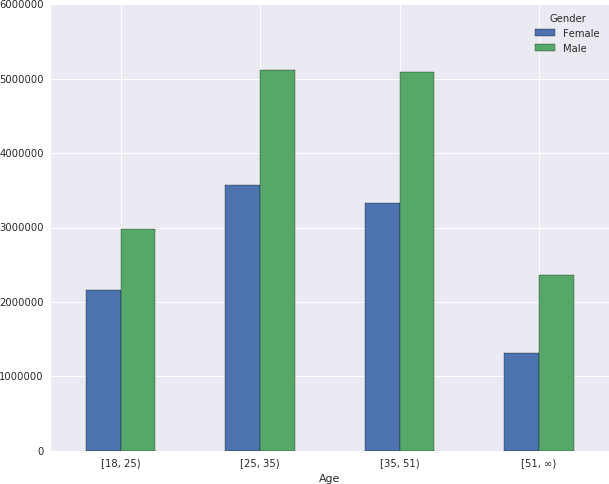
\includegraphics[width=0.9\columnwidth]{figures/gender_age_bar3/gender_age_bar3.png}
\caption{Amount of users in $B$ by gender and age.}
\label{fig:gender_age_bar}
\end{figure}

The demographic data can be easily combined with the income data to show income by age, as figured in Figure~\ref{fig:income_age_boxplot}. The data shows how the median income increases with age up to the age of retirement, at around 60--65 years, and later it rapidly decreases.

In another line of work, homophily with respect to age has been observed and used to generate inferences~\cite{brea2014}.

\begin{figure}
\centering
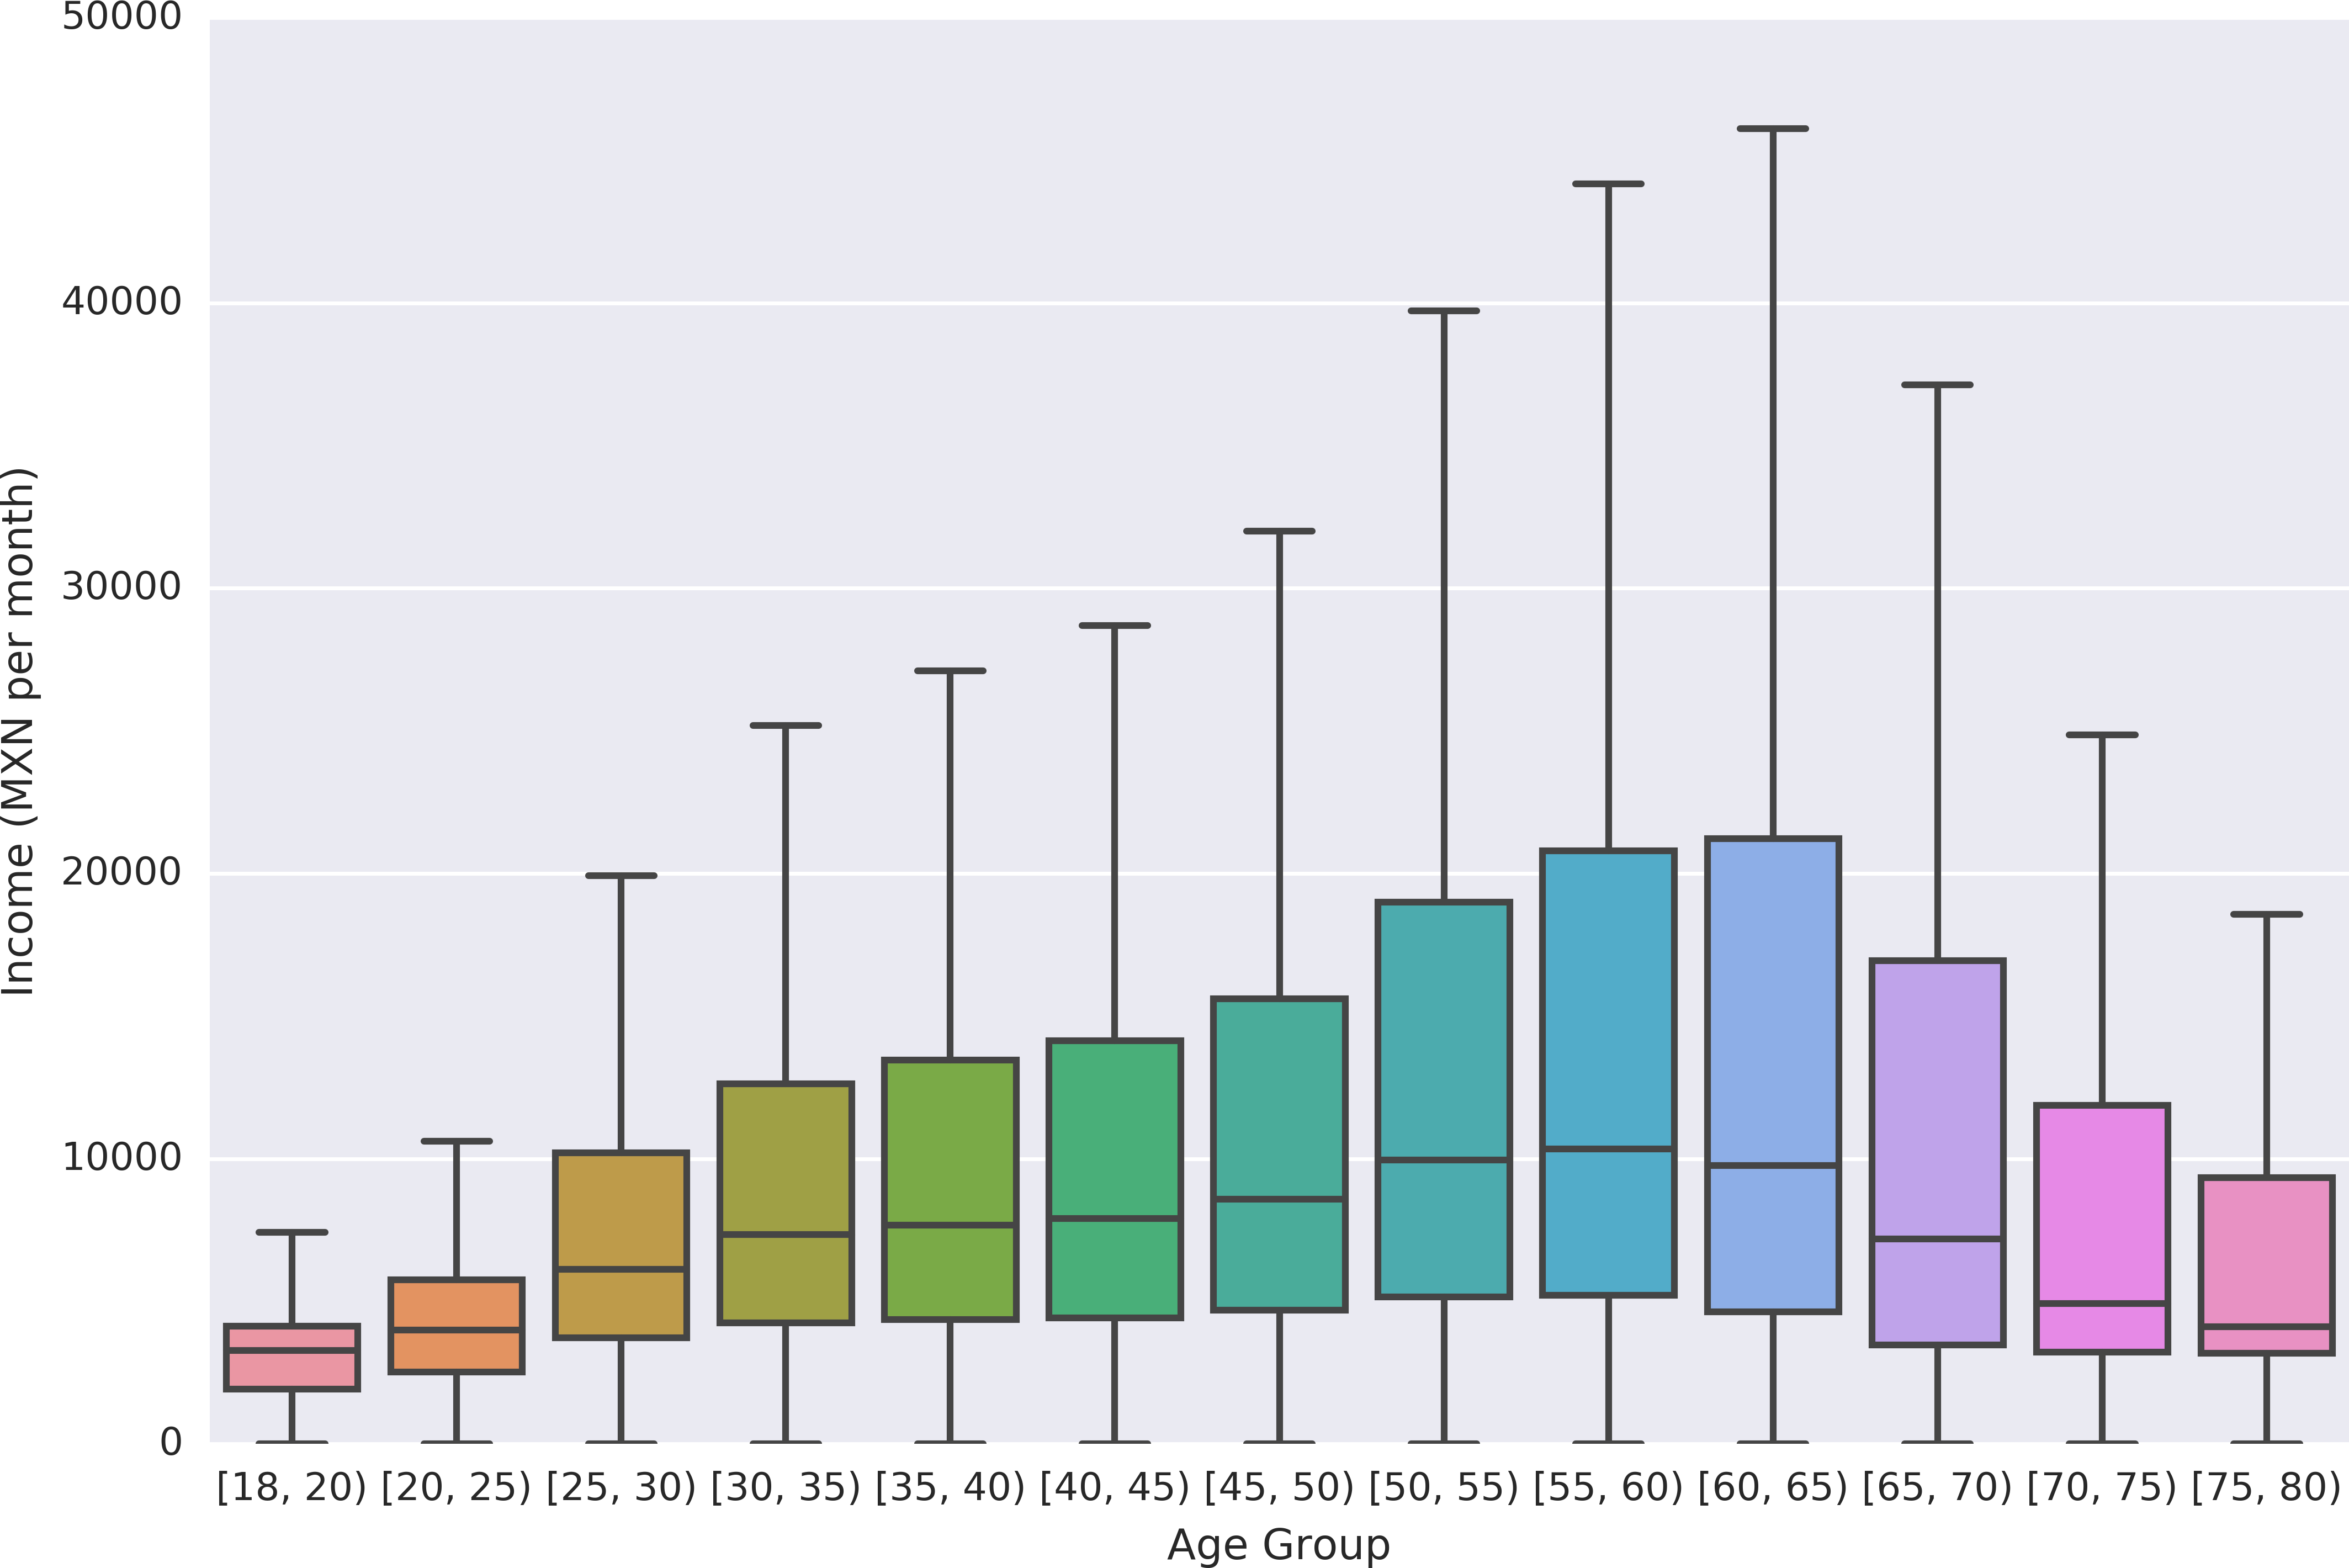
\includegraphics[width=0.9\columnwidth]{figures/income_age_boxplot4/income_age_boxplot4.png}
\caption{Distribution of income $a_s$ as a factor of age $a_a$. This is consistent with data from median house income in Mexico~\cite{gallup2013}.}
\label{fig:income_age_boxplot}
\end{figure}

The income distribution, as shown in \Cref{fig:income_distribution} presents a similar distribution to the values in the dataset presented in~\Cref{subsec:telco_magnitude}\maybe{Check this}.

\begin{figure}
\centering
\includegraphicsmaybe{figures/incomedistribution.png}
\caption{Distribution of incomes of users, represented by the set $B$}
\label{fig:income_distribution}
\end{figure}

\subsection{Matching of Bank and Telco Information}

Since the phone numbers in each call in the list of users $V$ are anonymized with the same hash function as the phone number in the bank data in the set $B$, the users can be matched to their unique phone to augment the \emph{Social Graph} $G$, where the elements in the set $S = V \cap B$ contain banking information.

\begin{equation}
\label{eq:banktelcojoin}
\begin{gathered}
G = \left< V, E \right> \\
( \forall e \in E ) \\
e_o = b_p \implies e_{\operatorname{so}} = b_s \\
e_d = b_p \implies e_{\operatorname{sd}} = b_s \\
\end{gathered}
\end{equation}

The distribution of bank users in $S$ is similar to the one in $B$, as shown in~\Cref{fig:matchdistribution}. This demostrates that the users of this particular telco have mostly the same socioeconomic patterns as the clients of the bank in general.

\begin{figure}
\centering
\includegraphicsmaybe{figures/matchdistribution.png}
\caption{Distribution of incomes for users of both the bank and telco, represented by the set $S$.}
\label{fig:matchdistribution}
\end{figure}


% \subsection{Outlier Filtering}
% 
% The dataset contains information about bank and telco users, some of which may not directly correspond to a human user, % who exclusively users the telco and the bank used in this study,
% or may not have useful information for our research.
% Most of the telco users in the first case are already filtered by the intersection (\textsc{inner join}). To make sure the users are relevant enough for this study, we only keep the users which have:
% 
% \begin{itemize}
% 	\item More than 5 calls in either direction.
% 	\item A monthly income of at least \$\num{1000}.
% 	The value is expressed in Mexican pesos (MXN)\footnote{At the time of writing (July 14, 2016), 1000 Mexican pesos are equivalent to 54 US dollars.}.
% 	\item A monthly income in the \num{99}th percentile (i.e.\ we filter users with a monthly income in the top 1\%).
% \end{itemize}

\subsection{Unequal Distribution of Income}

We provide here some observations of the distribution of income of the bank clients. These observations correspond to the filtered dataset, obtained after applying the filters of the previous section.

\Cref{fig:income_distribution} shows the Lorenz curve, graphical representation of the distribution of income~\cite{satchell1987}. The curve plots the cumulative share of clients, sorted by income, to the fraction of the total income of the population.

\begin{figure}
\centering
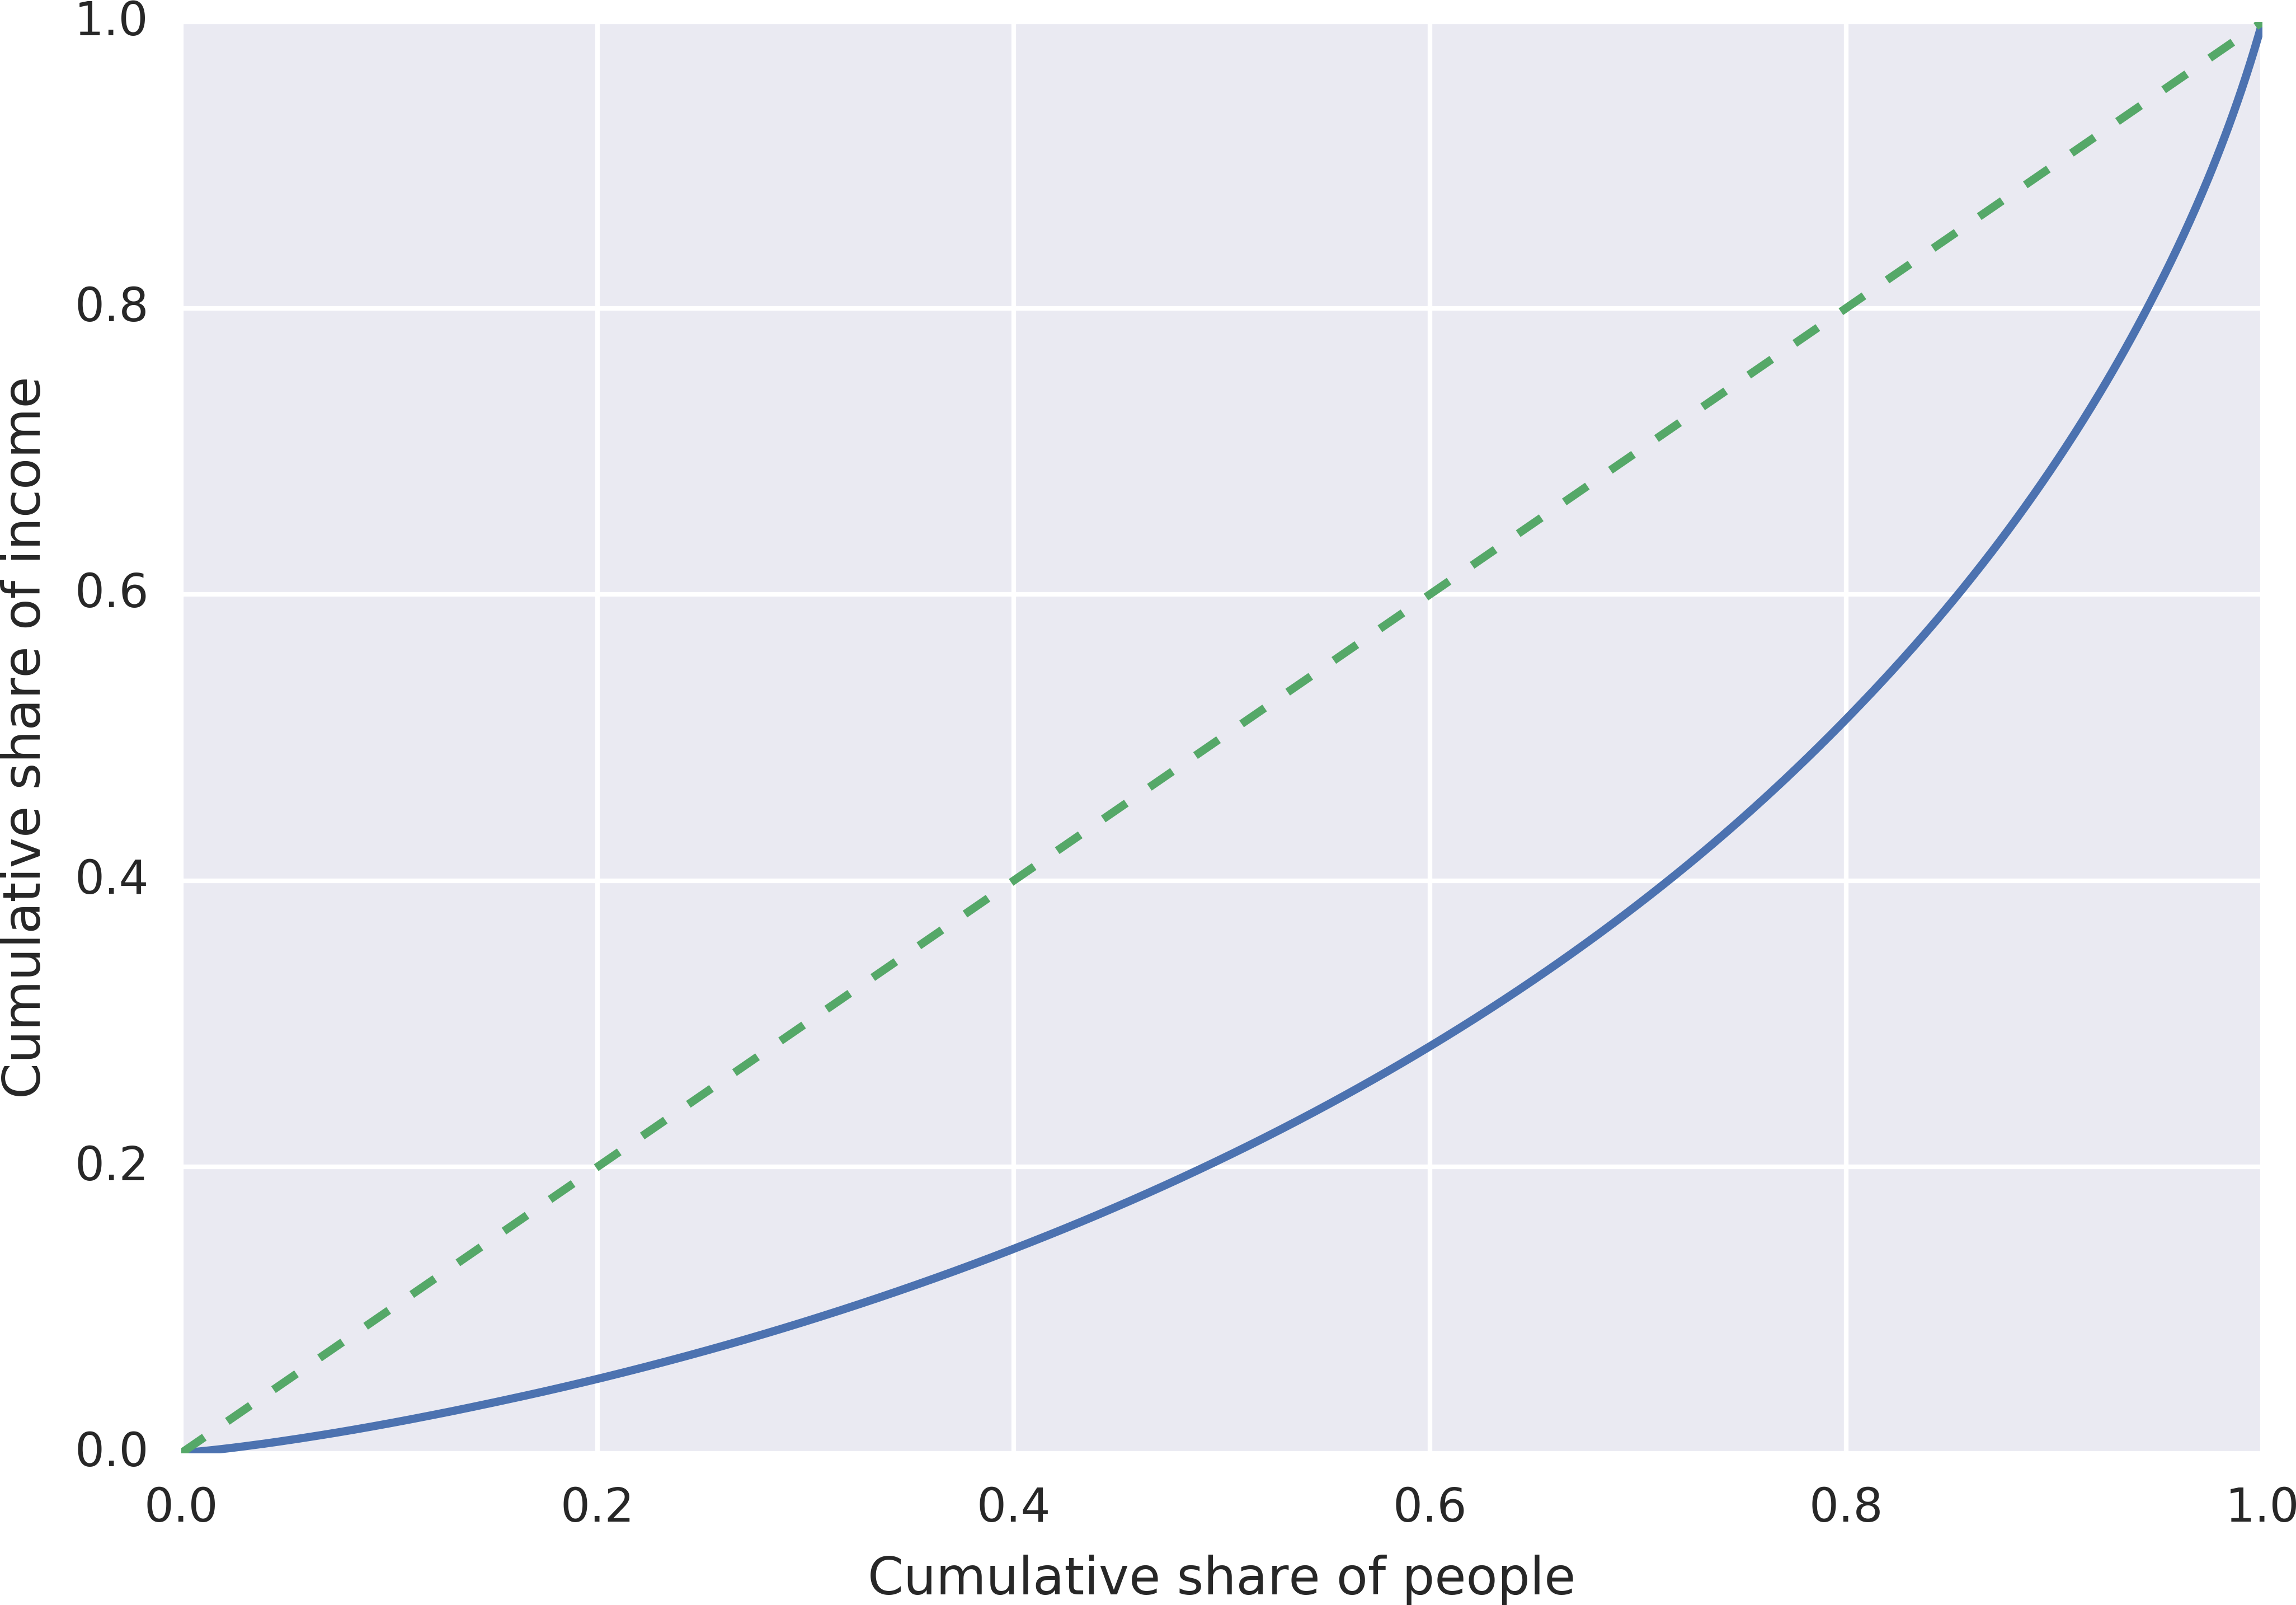
\includegraphics[width=0.9\columnwidth]{figures/cumulative_income.png}
\caption{Lorenz curve representing the distribution of income of bank clients.}
\label{fig:income_distribution}
\end{figure}

From the Lorenz curve, we can compute the Gini coefficient as the area that lies between the line of perfect equality and the Lorenz curve over the total area under the line of equality. The data presents a coefficient of $\operatorname{Gini} = 0.45$.

According to the World Bank~\cite{world_bank}, the Gini coefficient for the whole population of Mexico was $0.481$ in 2012. Our result is consistent with this information, since the income inequality is expected to be lower when accounting only to bank clients than within the whole population of the country.

Analyzing \Cref{fig:income_distribution}, we can observe that the top 10\% of the clients accumulate 33\% of the total income, while the top 20\% accumulate 50.5\% and the top 30\% accumulate 63.1\%; the rest of the income is distributed among the remaining 70\% of the population.

\subsection{Regional Distribution of Income}

Given the have locations of the calls in the subset $G' \subseteq G$, we can infer the home of each user in $V'$ using the method described in~\cite{csaji2013}. This is extremely useful when doing analyses, since it allows us to find differences in income distribution between areas of Mexico. In particular, \Cref{fig:regions} shows the average income per Mexican State in our dataset, which is compared to the data in Mexico in \Cref{tab:regions}.

\begin{figure}
\centering
\includegraphicsmaybe{figures/regions.png}
\caption{Average income by region of Mexico}
\label{fig:regions}
\end{figure}

\begin{table}[p]
\centering
\begin{tabular}{>{\bfseries}l c c c}
\toprule
\multirow{2}{*}{State} & \multirow{2}{*}{Count in dataset} & Average Income & Average Income \\
& & (current dataset) & (Mexico's census) \\
\midrule
Aguascalientes & & & \\
Baja California Norte & & & \\
Baja California Sur & & & \\
Campeche & & & \\
Chiapas & & & \\
Chihuahua & & & \\
Ciudad de México & & & \\
Coahuila & & & \\
Colima & & & \\
Durango & & & \\
Estado de México & & & \\
Guanajuato & & & \\
Guerrero & & & \\
Hidalgo & & & \\
Jalisco & & & \\
Michoacan & & & \\
Morelos & & & \\
Nayarit & & & \\
Nuevo Leon & & & \\
Oaxaca & & & \\
Puebla & & & \\
Queretaro & & & \\
Quintana Roo & & & \\
San Luis Potosi & & & \\
Sinaloa & & & \\
Sonora & & & \\
Tabasco & & & \\
Tamaulipas & & & \\
Tlaxcala & & & \\
Veracruz & & & \\
Yucatan & & & \\
Zacatecas & & & \\
\bottomrule
\end{tabular}
\caption{Income information about Mexico's regions}
\label{tab:regions}
\end{table}
